\documentclass[12pt]{article}
\usepackage{array}
\usepackage{amsmath}
\usepackage{mathtools}
\usepackage{gensymb}
\usepackage{graphicx}
\usepackage{float}
\usepackage{caption}
\usepackage{setspace}
\usepackage{multirow}

\allowdisplaybreaks

\begin{document}

    \title{Verificaiton of Bernoulli's Law}
    \author{Ryan Coyne, Ben Eid, Erin Snook}
    \maketitle

    \section{Abstract}
        Bernoulli's Law was tested using one liter soda bottles from which the bottoms had been removed. Each bottle had a different size outlet with diameter \(d\). The theoretical slope of the graph of the time to drain, \(T\), vs \(1/d^{2}\) was compared with the actual slope of the graph determined from the recorded data. The predicted slope was \((0.002489 \pm 0.000056) \mathrm{~s \cdot m^2}\) while the observed slope was \((0.002732 \pm 0.000053) \mathrm{~s \cdot m^2}\). The slopes were also compared for the graph of the acceleration, \(a_0^{1/4}\) vs \(d\). The predicted slope for this graph was \((16.61 \pm 0.18) \mathrm{~s^{1/2}/m^{3/4}}\) and the theoretical slope was \((16.74 \pm 0.041)\mathrm{~s^{1/2}/m^{3/4}}\).
    \section{Introduction}
        Bernoulli's principle says that an increase in a fluid's speed or height corresponds to a decrease in the fluid's pressure. This is reprsented mathematically as 
        \begin{equation*}
            p_1 + \frac{1}{2} \rho v_1^2 + \rho g h_1 = p_2 + \frac{1}{2} \rho v_2^2 + \rho g h_2
        \end{equation*}
        or
        \begin{equation*}
            p + \frac{1}{2} \rho v^2 + \rho g h = \text{constant}
        \end{equation*}
        where \(p\) is the fluid's pressure, \(\rho\) is it's density, \(v\) is it's velocity, \(g\) is the acceleration due to gravity, \(h\) is the fliud's height, and \(c\) is a constant.

        In this experiment, water flows downward from height where the bottle has a particular cross-sectional area to a height with a smaller cross-sectional area, and at both ends, the pressure is equal to atmospheric pressure because both are open to the air. The equation
        \begin{equation*}
            |v_1|A_1 = |v_2|A_2
        \end{equation*}
        is known in fluid dynamics as the equation of continuity, and it relates the velocity of a fluid to the cross-sectional area of the space it is flowing through, such that if the area decreases, then the speed should increase proportionally. 
    \section{Procedure}
        To begin with set out 3 straight metal rods, a digital motion sensor, 2 two-prong extension clamps, a bucket, a table clamp with a slot for a vertical rod, 2 right-angle clamps, and 3 two-liter plastic bottle's with the bottoms cut off, 3 bottle caps with holes of various diameters cut into them, a string, and a ruler. Screw a cap onto each bottle. Make a mark on one of the bottles near the large opening. Thread the string through the opening in the bottle cap and mark a length on the string that is the distance from mark to the point where the string exits the cap. Measure this length and use the same technique of threading the string through the cap to make a mark at the same distance on each bottle.
        
        Attach the table clamp to a table. Secure a metal rod vertically into the clamp, and place the bucket in front of it on the table. Attach an extension clamp directly to the vertical rod so that it is horrizontal and directly above the bucket. Secure one of the bottles into the clamp. Secure an angle clamp to the vertical rod and slot another rod into it so that it is horrizontal and above the bottle. Add an extension clamp to the new rod so that it is gripping the edge of the bottle to keep the bottle from moving. Use the last angle clamp to attach the last rod horrizontally above the previous rod. Affix the motion sensor to the newest rod so that it is facing downward and has an un-obstructed view of the inside of the bottle.

        Have one person plug the outlet in the cap with a finger and another fill the bottle with water up to the mark. Allow the water to settle, and then start recording from the motion sensor. Remove the finger that is obstructing the outlet. Once the water has drained stop recording. Remove the bottle and repeat the steps for each.

        \begin{figure}[H]
            \centering
            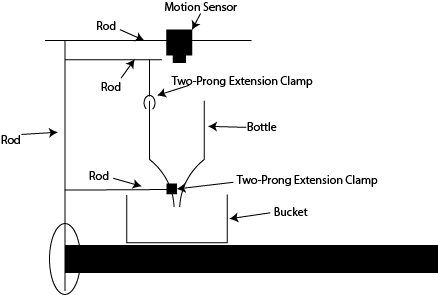
\includegraphics[width=0.75\linewidth]{setup.png}
            \caption{Experimental setup.}
        \end{figure}
    \section{Data}
        \begin{center}
            \begin{tabular}{c|c|c|c|c}
                Bottle & Trial & \(H\) & \(D\) (cm)& \(d\) (cm)\\
                \hline
                \multirow{3}{*}{1} & 1 & & 10.64 & 0.409\\
                & 2 &  & 10.55 & 0.645\\
                & 3 &  & 10.80 & 0.634\\
                \hline
                \multirow{3}{*}{2} & 1 & & 10.89 & 0.679\\
                & 2 &  & 10.60 & 0.658\\
                & 3 &  & 10.56 & 0.681\\
                \hline
                \multirow{3}{*}{3} & 1 & & 10.55 & 0.941\\
                & 2 &  & 10.60 & 0.816\\
                & 3 &  & 10.71 & 0.882\\
                \hline
                &\(\sigma_x\) & & 0.12
            \end{tabular}\\[6pt]
            Table 1: Bottle dimensions.\\[12pt]
            \begin{tabular}{c|c}
                \(\overline{H}\) (cm) & \(\overline{D}\) (cm)\\
                \hline
                0.235 & 10.66 
            \end{tabular}\\[6pt]
            Table 2: Average height and large diameter.\\[12pt]
            \begin{tabular}{c|c|c|c|c|c}
                Bottle & \(\overline{d}\) (cm)& \(T\) (s) & \(a_0~(\mathrm{m/s^2})\) & \(t_0\) (s) & \(y_0\) (m)\\
                \hline
                1 & 0.562 & 86.8 & \(0.0617\times10^{-32}\) & 2.06 & -0.244\\
                2 & 0.673 & 58.4 & \(0.135\times10^{3}\) & 1.68 & -0.250\\
                3 & 0.880 & 33.0 & \(0.420\times10^{-3}\) & 2.72 & -0.259\\
                4 & 2.113 & 5.67 & \(14.8\times10^{-3}\) & 2.56 & -0.234
            \end{tabular}\\[6pt]
            Table 3: ToDo
        \end{center}
        \begin{figure}[H]
            \centering
            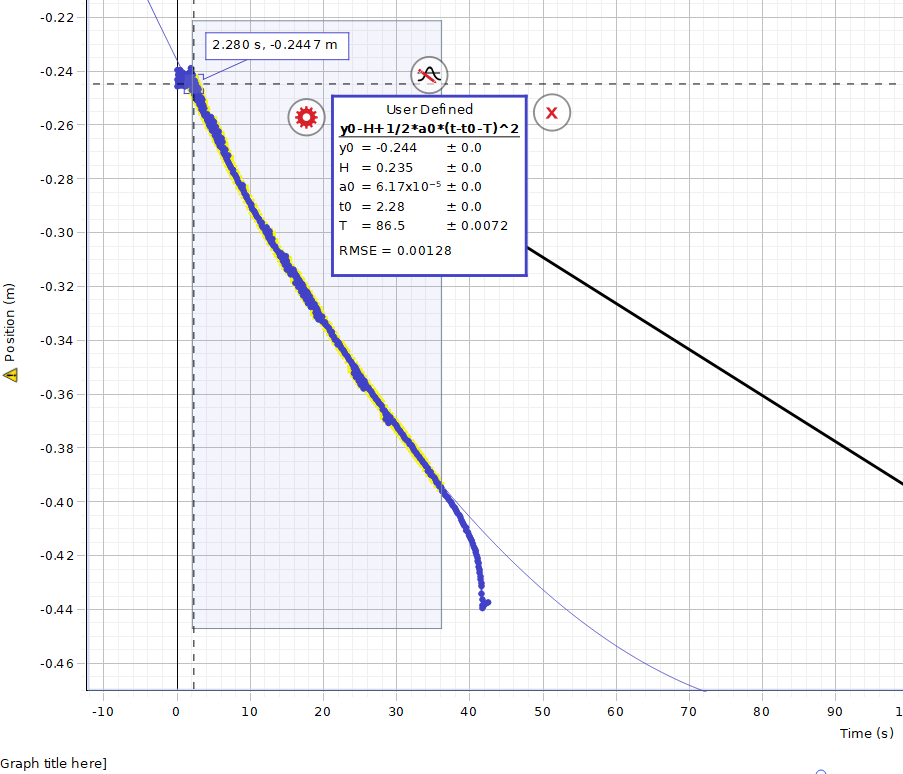
\includegraphics[width=0.9\linewidth]{y1.png}
            \caption{Plot of y vs t with (t0, y0) labeled and fit to find T, Bottle 1.}
        \end{figure}
        \begin{figure}[H]
            \centering
            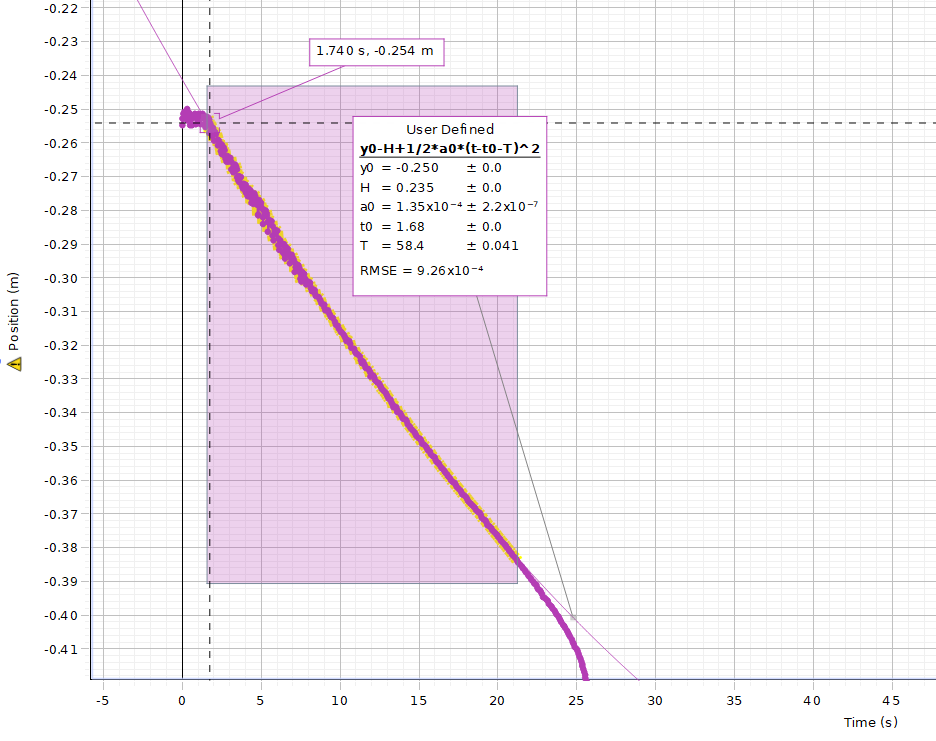
\includegraphics[width=0.9\linewidth]{y2.png}
            \captionsetup{justification=centering}
            \caption{Plot of y vs t with (t0, y0) labeled and fit to find T and a0, bottle 2.}
        \end{figure}
        \begin{figure}[H]
            \centering
            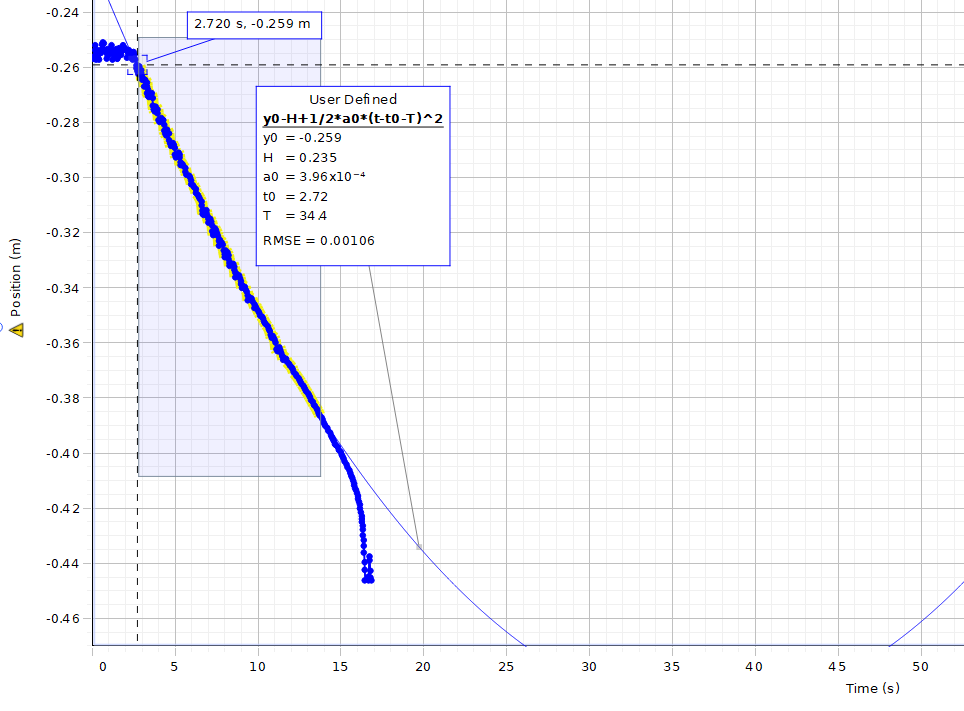
\includegraphics[width=0.9\linewidth]{y3.png}
            \captionsetup{justification=centering}
            \caption{Plot of y vs t with (t0, y0) labeled and fit to find T and a0, bottle 3.}
        \end{figure}
        \begin{figure}[H]
            \centering
            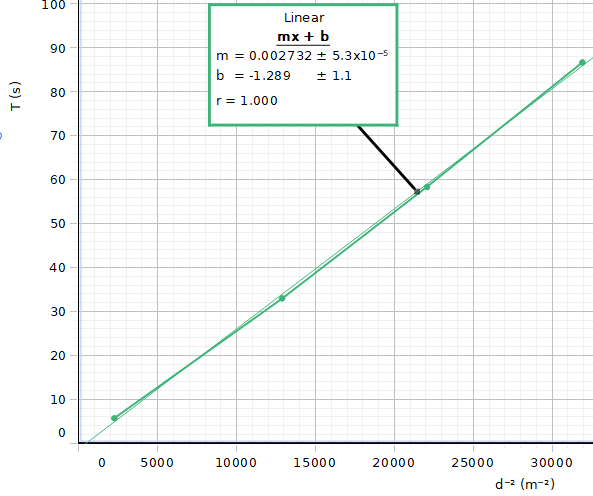
\includegraphics[width=0.9\linewidth]{fit1.png}
            \captionsetup{justification=centering}
            \caption{Plot of \(T\) vs \(1/d^2\) with linear fit. Predicted \((0.002489 \pm 0.000056) \mathrm{~s \cdot m^2}\).}
        \end{figure}
        \begin{figure}[H]
            \centering
            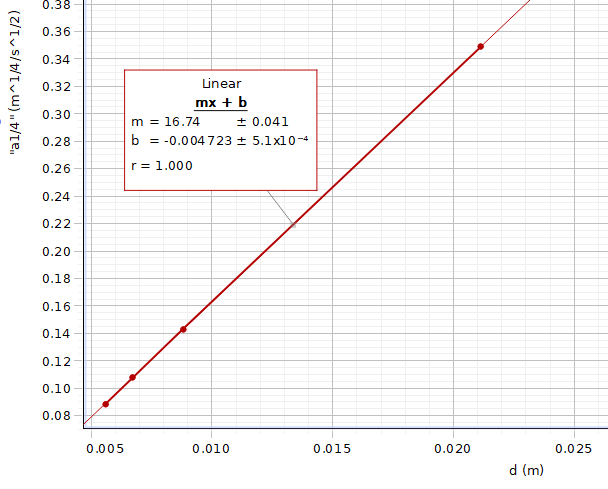
\includegraphics[width=0.9\linewidth]{fit2.png}
            \captionsetup{justification=centering}
            \caption{Plot of \(a_0^{1/4}\) vs \(d\) with linear fit. Predicted \((16.61 \pm 0.18) \mathrm{~s^{1/2}/m^{3/4}}\).}
        \end{figure}
    \section{Calculations}
        \begin{alignat*}{3}
            (1)~&&
            y&=y_2 + \frac{1}{2}a_0(\Delta t - T)^2\\
            &&&= y_0 - H + \frac{1}{2}a_0(t-t_0 - T)^2\\
            (2)~&&
            T&=\sqrt{\frac{2H}{a_0}}\\
            &&&\approx \sqrt{\frac{2H}{g(D/D)^4}}\\
            &&&\approx \frac{D^2}{d^2}\sqrt{\frac{2H}{g}}\\
            (3)~&&
            p+\frac{1}{2} \rho v^2 + \rho g y &= p_2 + \frac{1}{2} \rho v_2^2 + \rho g y_2\\
            &&p = p_2 &= p_{atm}\\
            &&v^2 + 2g y &= v_2^2+ 2 g y_2\\
            &&v_2^2-v^2 &= 2\rho g (y-y_2)\\
            &&|v|A_0 &= |v_2|A_2\\
            &&|v|\pi D^2 &= |v_2|\pi d^2\\
            &&|v_2| &= |v|\frac{D^2}{d^2}\\
            &&v^2\left( \frac{D}{d} \right)^4-v^2 &= 2\rho g (y-y_2)\\
            && v^2 &= 2\frac{g}{(D/d)^4-1}(y-y_2)\\
            &&a_0 &= \frac{g}{(D/d)^4-1}\\
            &&&=\frac{g}{1-(d/D)^4}\left(\frac{d}{D}\right)^4\\
            &&&\approx g\left(\frac{d}{D}\right)^4 \text{ for } d\ll D\\
            &&a_0^{1/4} & \approx \frac{g^{1/4}d}{D}\\
            (4)~&&
            \overline{S}_T&=D^2\sqrt{\frac{2H}{g}}\\
            &&&=(0.10655 \text{ m})^2\sqrt{\frac{2\cdot 0.235 \text{ m}}{9.8 \mathrm{~m/s^2}}}\\
            &&& = 0.002489\mathrm{~s \cdot m^2}\\
            &&S_{TD} &= (0.10655 + 0.0012\text{ m})^2\sqrt{\frac{2\cdot 0.235 \text{ m}}{9.8 \mathrm{~m/s^2}}}\\ 
            &&& = 0.002545\mathrm{~s \cdot m^2}\\
            &&\sigma_{S_T} &= 0.002545 \mathrm{~s \cdot m^2} -0.002489 \mathrm{~s \cdot m^2}\\
            &&&=5.6\times 10^{-5} \mathrm{~s \cdot m^2}\\
            (5)~&&
            \overline{S}_a &= \frac{g^{1/4}}{D}\\
            &&& = \frac{(9.8\mathrm{~m/s^2})^{1/4}}{0.10655\text{ m}}\\
            &&&= 16.61 \mathrm{~s^{1/2}/m^{3/4}}\\
            &&S_{aD} &= \frac{(9.8\mathrm{~m/s^2})^{1/4}}{(0.10655 + 0.0012)\text{ m}}\\
            &&&= 16.42 \mathrm{~s^{1/2}/m^{3/4}}\\
            &&\sigma_{S_a} &= 16.61 \mathrm{~s^{1/2}/m^{3/4}} - 16.42 \mathrm{~s^{1/2}/m^{3/4}}\\
            &&&=0.18\mathrm{~s^{1/2}/m^{3/4}}
        \end{alignat*}
    \section{Conclusion}
    The predicted slope of the graph of \(T\) vs \(1/d^2\) was \((0.002489 \pm 0.000056) \mathrm{~s \cdot m^2}\) while the observed slope was \((0.002732 \pm 0.000053) \mathrm{~s \cdot m^2}\). These slopes are separated by about four times the standard deviation of either value, but about twice the sum of their standard deviations. This seems reasonably close. The predicted slope for the graph of \(a_0\) vs \(d\) was \((16.61 \pm 0.18) \mathrm{~s^{1/2}/m^{3/4}}\) and the theoretical slope was \((16.74 \pm 0.041)\mathrm{~s^{1/2}/m^{3/4}}\). These slopes are within a single standard deviation which is certainly reasonable. Some error was likely introduced because of structural instability in the setup of the experiement. My thumb was also not a perfect seal on the outlet so there was water constantly leaking out before the actual release. Lastly the bottles are made of flexible plastic which deformed to some degree because of the weight of the water which could have added inaccuracy to the value of \(D\).
\end{document}